\documentclass[]{standalone}
\usepackage{tikz}
\usepackage{marvosym}
\usetikzlibrary{decorations.pathmorphing}
\usetikzlibrary{shapes}
\begin{document}
  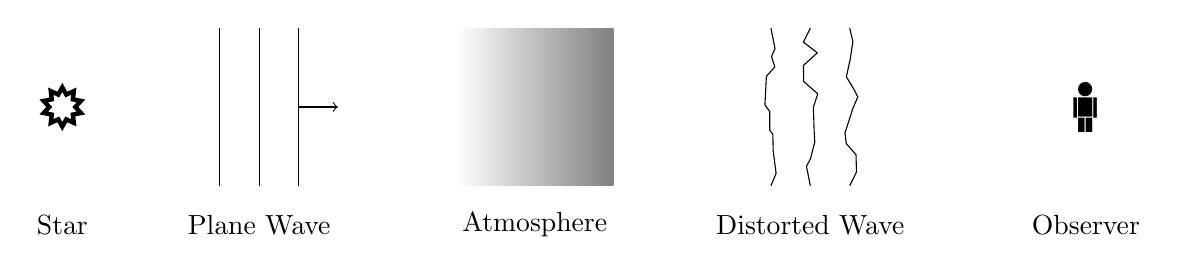
\begin{tikzpicture}
	%Star
    \tikzstyle{ann} = [draw=none,fill=none,right]
	\node[draw, ultra thick,star,star points=10] at (-2,-1){};
	\node at (-2,-2.5) {Star};
	%Plane Wave
	\draw (0,0) -- (0,-2);
	\draw (.5,0) -- (.5,-2);
	\draw (1,0) -- (1,-2);
	\draw[->] (1,-1) -- (1.5,-1);
	\node at (.5,-2.5) {Plane Wave};
	
	%Atmosphere
	\shade[left color = white, right color = gray] (3,-2) rectangle (5,0);
	\node at (4,-2.5) {Atmosphere};

	%Distorted Wave
	\draw [black, decorate, decoration={random steps,segment length=5pt,amplitude=3pt}] (7,0) to (7,-2);
	\draw [black, decorate, decoration={random steps,segment length=5pt,amplitude=3pt}] (7.5,0) to (7.5,-2);
	\draw [black, decorate, decoration={random steps,segment length=5pt,amplitude=3pt}] (8,0) to (8,-2);
	\node at (7.5,-2.5) {Distorted Wave};

	%observer
	\node at (11,-1) {\Huge \Gentsroom};
	\node at (11,-2.5) {Observer};

  \end{tikzpicture}
\end{document}
